\documentclass[10pt,a4paper]{article}
\usepackage[T1]{fontenc}
\usepackage{lmodern}
\usepackage{microtype}
\usepackage[margin=1.6cm,top=1.3cm,bottom=1.2cm]{geometry}
\usepackage{graphicx}
\usepackage{enumitem}
\usepackage[colorlinks=true,urlcolor=blue]{hyperref}
\pagestyle{empty}
\setlist{itemsep=2pt,topsep=2pt,leftmargin=14pt}
\setlength{\parindent}{0pt}
\setlength{\emergencystretch}{2em}
\setlength{\parskip}{4pt}
\newcommand{\head}[1]{\vspace{3pt}{\large\bfseries #1}\par\vspace{1pt}}

\begin{document}

{\LARGE\bfseries Momentum, Reversal, Volatility and Size in U.S.\ Large Caps}\par
\vspace{2pt}
{\large A cross-sectional factor study with Fama-MacBeth validation, 2011 to 2026: one-page summary}\par
\vspace{2pt}
Zack Higham, BSc Mathematics, Queen Mary University of London. Full paper (23 pages) and code:\par{\small\href{https://github.com/zack-higham/Cross-Sectional-Factor-Research-with-Fama-MacBeth-Validation}{github.com/zack-higham/Cross-Sectional-Factor-Research-with-Fama-MacBeth-Validation}}

\head{Question}
Do four standard characteristics (12-1 momentum, one-month reversal, 60-day volatility, log market capitalisation) predict next-month returns among the 200 largest S\&P 500 stocks, and which apparent premia survive risk adjustment, costs and checks for sample-construction bias?

\head{Data and method}
\begin{itemize}
\item \textbf{Data:} daily adjusted prices from January 2011; monthly returns to August 2026 (175 months with all four factors); SPY and T-bills for the market; Fama-French five factors and UMD; historical S\&P 500 membership lists.
\item \textbf{Three lenses:} equal-weighted decile long-short portfolios, Fama-MacBeth regressions with Newey-West $t$-statistics, and rank information coefficients, all on one timing convention (factor at end of $t-1$, return over $t$).
\item \textbf{Validation:} out-of-sample split, CAPM and Fama-French five-factor plus momentum alphas, 10 bps costs, drawdowns, sector neutrality, VIX regimes, a point-in-time membership filter and unwinsorised factors, the last four specified in advance and committed before being run.
\end{itemize}

\head{Findings}
\begin{enumerate}
\item \textbf{Momentum is the one robust premium, and it is the standard momentum factor.} Market-adjusted Fama-MacBeth premium 3.7\% a year per standard deviation ($t = 3.41$; $t = 2.49$ before 2023), significant under point-in-time membership ($t = 2.26$) and without winsorisation ($t = 3.64$). It loads heavily on UMD ($t = 8.83$), and its alpha beyond UMD before 2023 is insignificant ($t = 1.01$). The decile portfolio lost 56.3\% from January 2016 to May 2023.
\item \textbf{The volatility premium is not a usable premium.} Raw Fama-MacBeth $t = 3.07$, but the long-short portfolio has a market beta of 1.17 and an insignificant CAPM alpha ($-3.13\%$ a year before 2023). Its FF5+UMD alpha of 15.95\% a year ($t = 3.51$) comes from loading on unprofitable, heavily investing firms ($-1.75$ on RMW) that nonetheless won: the signature of ex post selection. The residual volatility premium loses significance under point-in-time membership ($t = 3.05$ to $1.79$).
\item \textbf{Size and reversal are not findings.} The big-minus-small spread ($-21.26\%$ a year) is survivorship bias from an end-of-sample universe; the point-in-time filter shrinks it by 25.4\%, a partial confirmation under the pre-set rule. Reversal's turnover (3.44 a month) puts its break-even cost at 9.7 bps, so it does not survive costs.
\end{enumerate}

\begin{center}
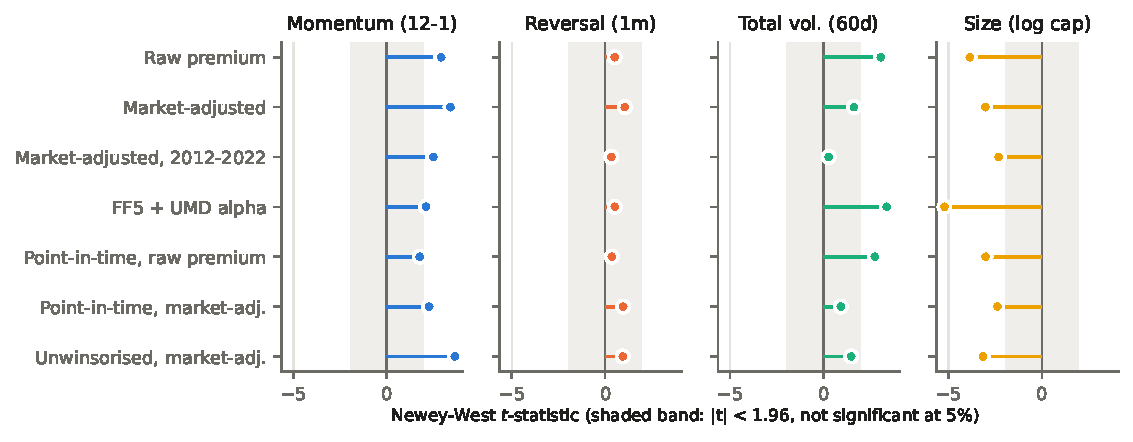
\includegraphics[width=0.93\textwidth]{figures/robustness_summary.pdf}\\[-2pt]
{\small Fama-MacBeth $t$-statistic of each factor across specifications. Momentum is the only positive premium significant in every specification; size is significantly negative throughout, which reflects survivorship bias rather than a size effect.}
\end{center}

\head{Main limitation}
The universe is the September 2026 top 200, applied to the whole history. The point-in-time filter removes stocks from months before they joined the index, but firms that left it (acquired, shrank, failed) are still missing, so the remaining survivorship bias is smaller but not zero. Results rest on 175 months and about 20 stocks per decile, and no premium outside 2023 to 2026 clears the $t > 3$ multiple-testing hurdle.

\end{document}
